\documentclass{article}

\usepackage{graphicx}
\usepackage{tikz}
\usepackage{tikzsymbols}
\usetikzlibrary{calc,patterns,shapes.geometric}
\pagestyle{empty}
\usepackage[margin=0pt]{geometry}
\geometry{papersize={14in,12in}}

\def\centerarc[#1](#2)(#3:#4:#5){\draw[#1] ($(#2)+({#5*cos(#3)},{#5*sin(#3)})$) arc (#3:#4:#5);}

\begin{document}
	\begin{figure}
		\centering
		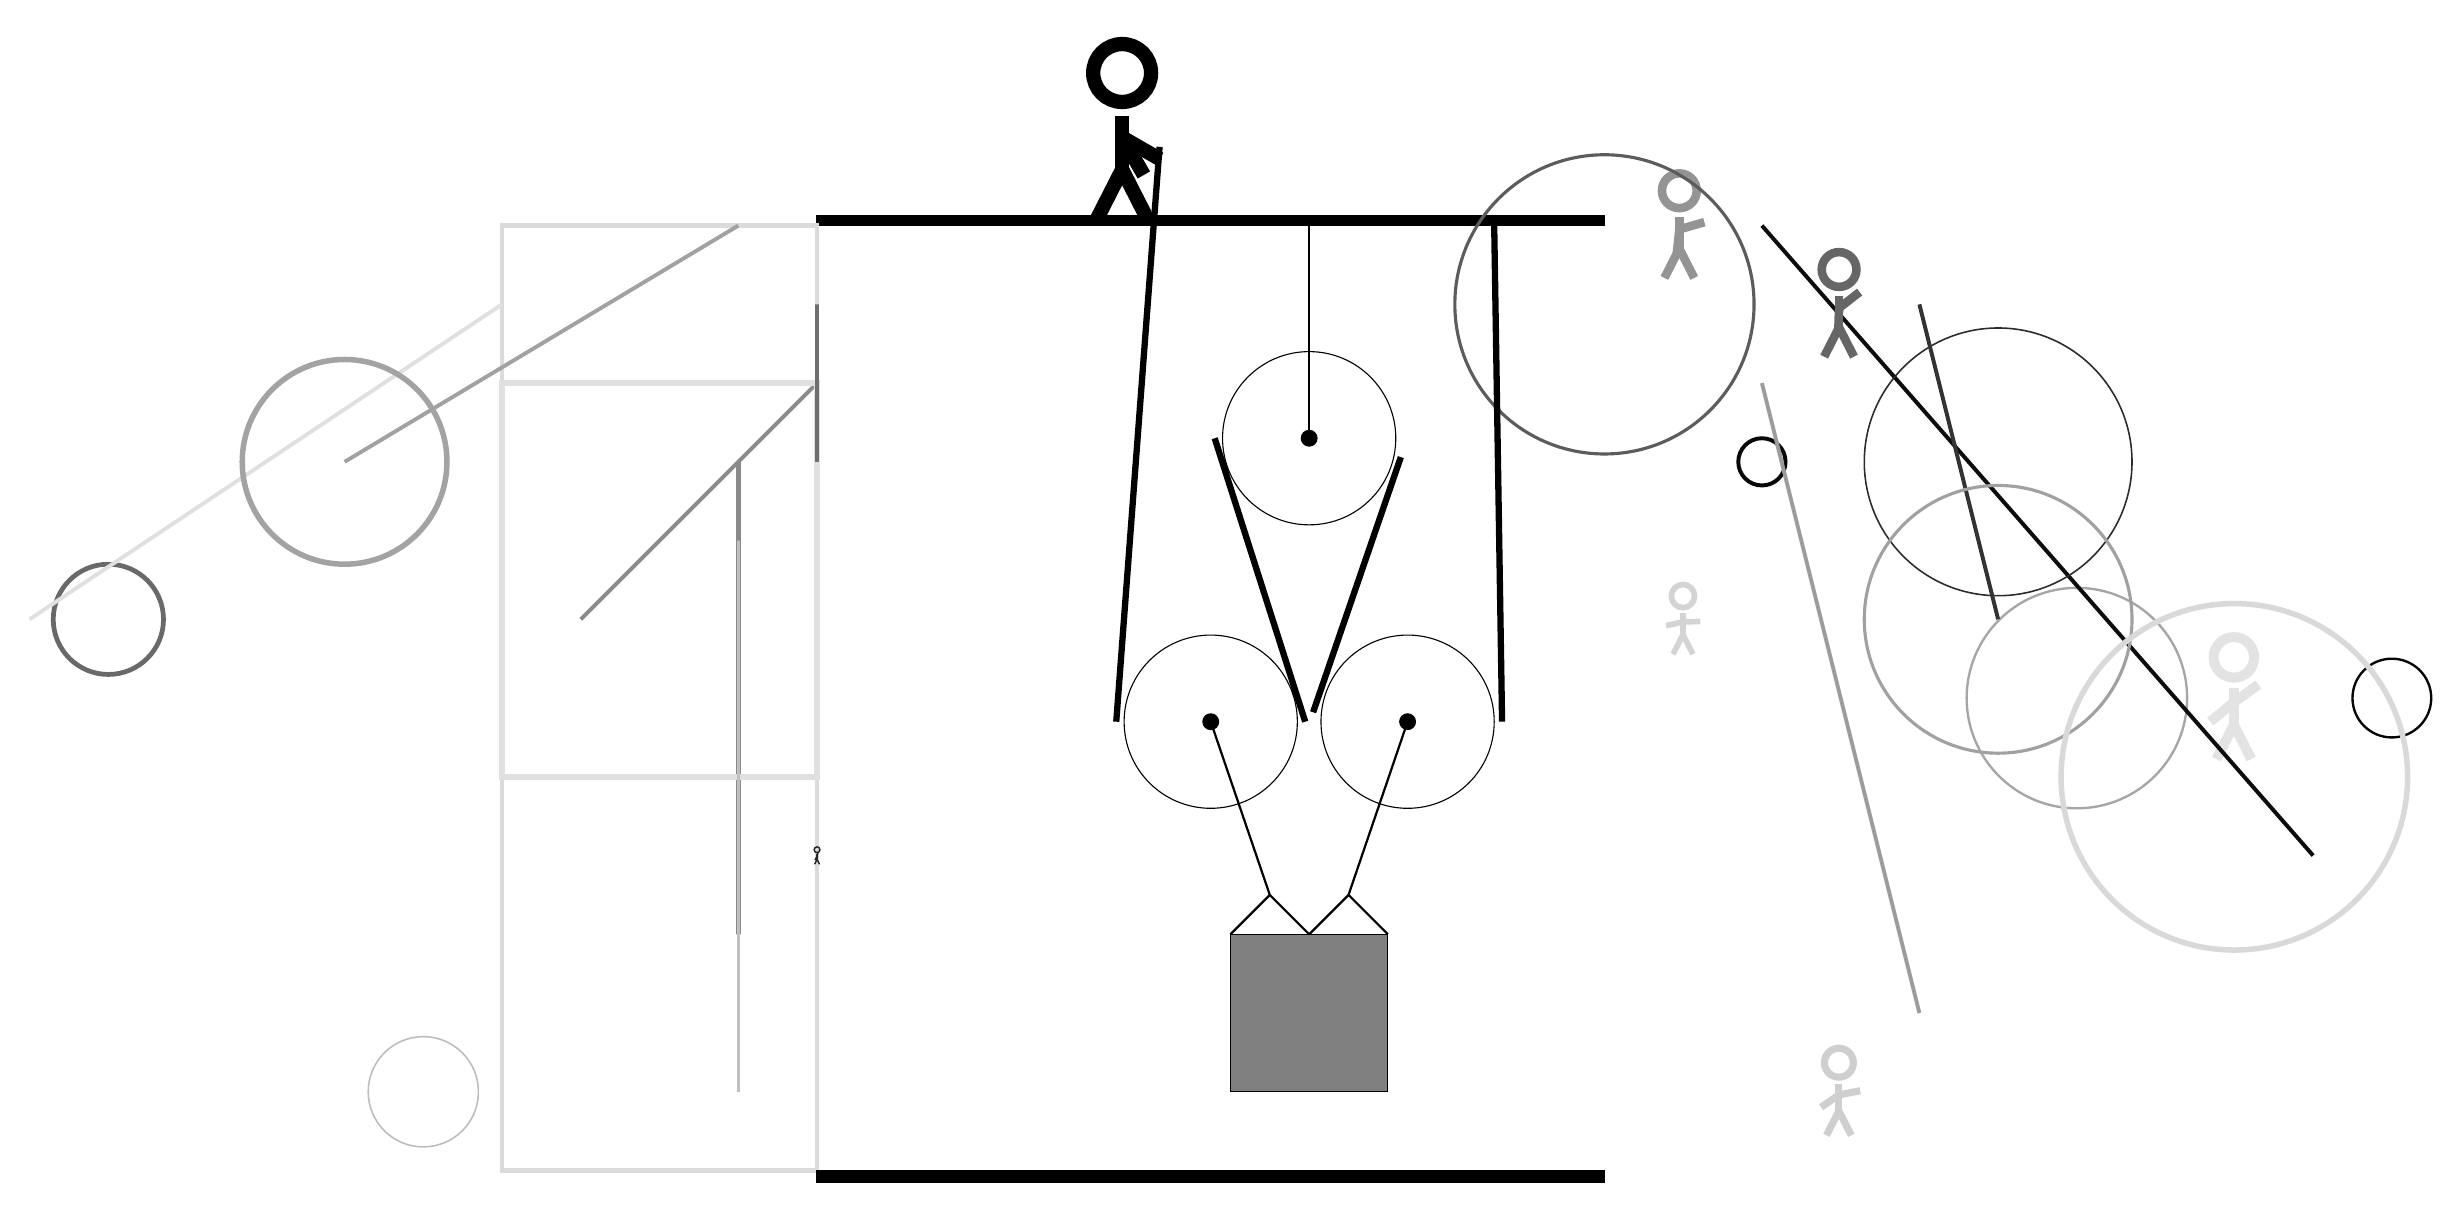
\begin{tikzpicture}
			%%%%% START %%%%%
			
			\draw[fill=black] (-4, 9) rectangle (6, 9.125);
			
			\draw (1, 2.7) circle (1.1);
			\draw[fill=black] (1, 2.7) circle (0.1);
			
			\draw (2.25, 6.3) circle (1.1);
			\draw[fill=black] (2.25, 6.3) circle (0.1);
			\draw[thick] (2.25, 6.3) -- (2.25, 9);
			
			\draw [line width=0.3mm, color=black!35](12, 3) circle (1.4);
			
			\node[line width=0.2mm, color=black!11] at (14, 3) {\Strichmaxerl[7][39][36]};
			\draw[line width=0.5mm, color=black!95](8, 9) -- (15, 1);
			\draw[line width=0.5mm, color=black!46](-4, 7) -- (-7, 4);
			
			\node[line width=0.6mm, color=black!17] at (7, 4) {\Strichmaxerl[4][13][1]};
			\draw[line width=0.6mm, color=black!14] (-4, -3) rectangle (-8, 9);
			
			\node[line width=0.5mm, color=black!86] at (-4, 1) {\Strichmaxerl[1][63][76]};
			\node[line width=0.2mm, color=black!42] at (7, 9) {\Strichmaxerl[6][84][16]};
			\draw [line width=0.6mm, color=black!59](-13, 4) circle (0.7);
			\draw [line width=0.4mm, color=black!64](6, 8) circle (1.9);
			\draw [line width=0.2mm, color=black!83](11, 6) circle (1.7);
			\draw[line width=0.5mm, color=black!12](-8, 8) -- (-14, 4);
			\draw [line width=0.3mm, color=black!98](16, 3) circle (0.5);
			\draw[line width=0.5mm, color=black!37](-5, 9) -- (-10, 6);
			\draw[line width=0.5mm, color=black!80](11, 4) -- (10, 8);
			\draw[line width=0.6mm, color=black!46] (-5, 6) rectangle (-5, 0);
			\draw [line width=0.5mm, color=black!97](8, 6) circle (0.3);
			\node[line width=0.2mm, color=black!19] at (9, -2) {\Strichmaxerl[5][35][11]};
			\draw[line width=0.7mm, color=black!12] (-4, 7) rectangle (-8, 2);
			\node[line width=0.3mm, color=black!60] at (9, 8) {\Strichmaxerl[6][88][38]};
			\draw[line width=0.4mm, color=black!25] (-5, -2) rectangle (-5, 5);
			
			\draw[line width=0.5mm, color=black!39](10, -1) -- (8, 7);
			
			\draw [line width=0.7mm, color=black!36](-10, 6) circle (1.3);
			\draw [line width=0.2mm, color=black!26](-9, -2) circle (0.7);
			\draw[line width=0.5mm, color=black!57] (-4, 6) rectangle (-4, 8);
			\draw [line width=0.4mm, color=black!37](11, 4) circle (1.7);
			\draw [line width=0.7mm, color=black!15](14, 2) circle (2.2);
			
			\draw (3.5, 2.7) circle (1.1);
			\draw[fill=black] (3.5, 2.7) circle (0.1);
			
			\draw[thick] (3.5, 2.7) -- (2.75, 0.5);
			\draw[thick] (1, 2.7) -- (1.75, 0.5);
			\draw[thick]  (1.25, 0) -- (1.75, 0.5) -- (2.25, 0);
			\draw[thick]  (2.25, 0) -- (2.75, 0.5) -- (3.25, 0);
			\draw[fill=black!50] (1.25, 0) rectangle (3.25, -2);
			
			\draw[line width=0.8mm] (0.35, 10) --  (-0.2, 2.7);
			\centerarc[line width=0.8mm](1, 2.7)(180:360:1.2000000000000002);
			\draw[line width=0.8mm] (2.2, 2.7) -- (1.05, 6.3);
			\centerarc[line width=0.8mm](2.25, 6.3)(-20:180:1.2000000000000002);
			\draw[line width=0.8mm](3.414, 6.06) -- (2.3, 2.82);
			\centerarc[line width=0.8mm](3.5, 2.7)(160:360:1.2000000000000002);
			\draw[line width=0.8mm](4.7, 2.7) -- (4.6, 9);
			
			\node at (-0.07, 10.2) {\Strichmaxerl[10][120][-30]};
			
			\draw[fill=black] (-4, -3) rectangle (6, -3.15);
			
			%%%%% END %%%%%
		\end{tikzpicture}
	\end{figure}	
\end{document}